\section{Lei de Coulomb}

\frame{
	\frametitle{Lei de Coulomb}
	\begin{block}{Definição}
		Esta lei, em 1725, formulada por Charles Augustin Coulomb, faz uma relação entre a intensidade da força eletrostática entre duas \textbf{cargas elétricas puntiformes}, ou seja, com dimensão e massa desprezíveis.
	\end{block}
	
	\medskip

	\centerline{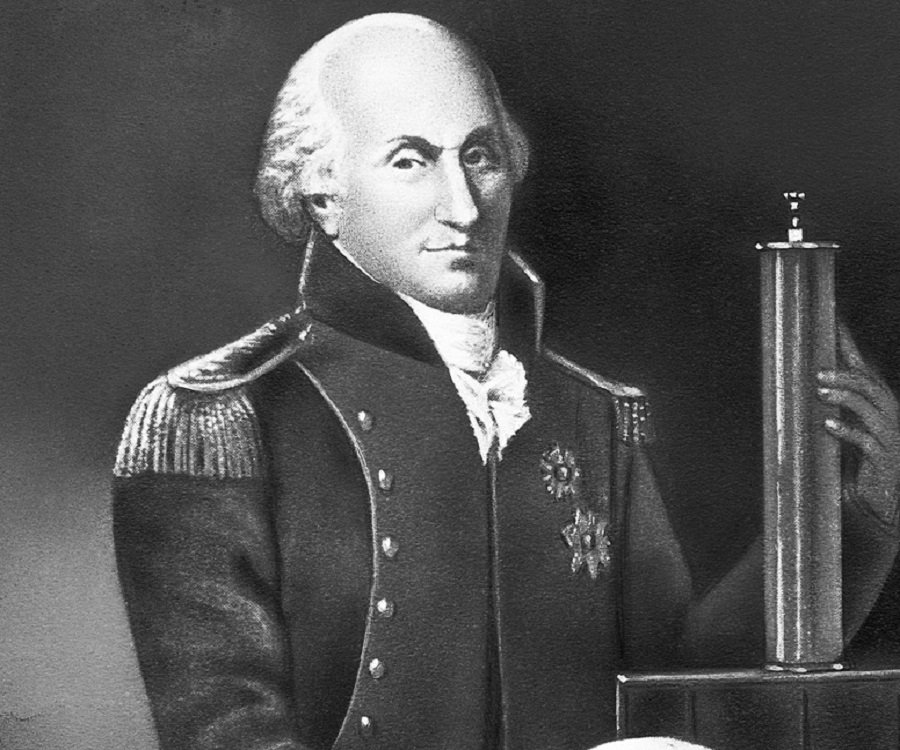
\includegraphics[width=0.45\linewidth]{Figuras/Ch05/coulomb.jpg}}
}

\frame{
	\frametitle{Lei de Coulomb}
	\begin{block}{Forças de atração e repulsão}
		Se as cargas das partículas têm o mesmo sinal, as partículas se repelem, ou seja, são submetidas a \textbf{forças que tendem a afastá-las}. Se as cargas das partículas têm sinal opostos, as partículas se atraem, ou seja, são submetidas a \textbf{forças que tendem a aproximá-las}.
	\end{block}

	\setmyunit{1.5cm}

	\centering
	\begin{tikzpicture}
		\draw (0,0) circle (0.25) node {$ + $} (2,0) circle (0.25) node {$ + $}
			(0,-1) circle (0.25) node {$ - $} (2,-1) circle (0.25) node {$ - $}
			(0,-2) circle (0.25) node {$ + $} (2,-2) circle (0.25) node {$ - $};
		\draw[-Latex] (-0.25,0) -- node[midway,below] {$ -F_e $} ++(-0.5,0);
		\draw[-Latex] (2.25,0) -- node[midway,below] {$ F_e $} ++(0.5,0);
		
		\draw[|-|] (0,-0.5) -- node[midway,below] {$ d $} (2,-0.5);
		
		\draw[-Latex] (-0.25,-1) -- node[midway,below] {$ -F_e $} ++(-0.5,0);
		\draw[-Latex] (2.25,-1) -- node[midway,below] {$ F_e $} ++(0.5,0);
		
		\draw[|-|] (0,-1.5) -- node[midway,below] {$ d $} (2,-1.5);
		
		\draw[-Latex] (0.25,-2) -- node[midway,below] {$ F_e $} ++(0.5,0);
		\draw[-Latex] (1.75,-2) -- node[midway,below] {$ -F_e $} ++(-0.5,0);
		
		\draw[|-|] (0,-2.5) -- node[midway,below] {$ d $} (2,-2.5);
	\end{tikzpicture}
%	\centerline{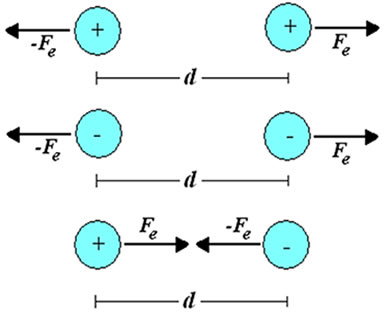
\includegraphics[width=0.5\linewidth]{Figuras/Ch05/coulomb2.jpg}}
}

\frame{
	\frametitle{Lei de Coulomb}
	\begin{block}{Experimento}
		Coulomb construiu um aparelho denominado balança de torção, através do qual ele podia fazer medidas da força de atração e repulsão entre duas esferas eletricamente carregadas. Nessa balança construída por Coulomb há uma haste que é suspensa por um fio e em cada uma de suas extremidades há uma esfera. Tomando outra haste com uma esfera também eletrizada, faz a aproximação entre as duas. Em razão da força elétrica que se manifesta nesse processo, a haste que está suspensa por um fio gira, provocando uma torção no fio. Ao medir o ângulo de torção, Coulomb conseguia determinar a força entre as esferas.
	\end{block}
}

\frame{
	\frametitle{Lei de Coulomb}
	\centerline{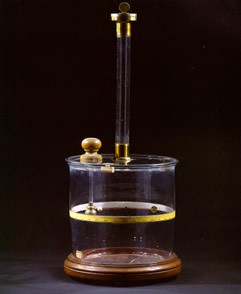
\includegraphics[width=0.5\linewidth]{Figuras/Ch05/balanca.jpg}}
}

\frame{
	\frametitle{Lei de Coulomb}
	\begin{block}{Formulação}
		\textit{``A força de ação mútua entre dois corpos carregados (cargas elétricas puntiformes) tem a direção da linha que une os corpos e sua intensidade é diretamente proporcional ao produto das cargas e inversamente proporcional ao quadrado da distância que as separa''.}
		
		$$F \propto \dfrac{Q_1 \ Q_2}{d^2}$$
	\end{block}
}

\frame{
	\frametitle{Lei de Coulomb}
	\begin{block}{Constante de proporcionalidade}
		A equação pode ser expressa por uma igualdade se considerarmos uma constante $K$, que depende do meio onde as cargas são encontradas. O valor mais usual de $K$ é considerado quando esta interação acontece no vácuo, e seu valor é igual a:
		
		$$K = \SI{9e9}{\newton\meter\squared\per\coulomb\squared} $$
	\end{block}
}

\frame{
	\frametitle{Lei de Coulomb}
	\begin{block}{Formulação}
		Então podemos escrever a equação da lei de Coulomb como:
		$$\boxed{F = K \ \dfrac{Q_1 \ Q_2}{d^2}}$$
	\end{block}
}

\frame{
	\frametitle{Lei de Coulomb}
	\begin{block}{Relação não linear}
		Se, a uma distância $d$, a intensidade da força é $F$, caso a distância passe a $2d$, a intensidade da força passará a ser $F/4$; e assim por diante.
	\end{block}
	
	\centering
	\scalebox{1.5}{

\tikzset{every picture/.style={line width=0.75pt}} %set default line width to 0.75pt        

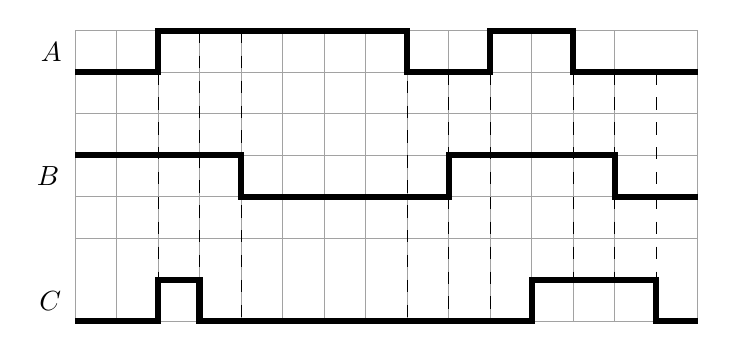
\begin{tikzpicture}[x=0.75pt,y=0.75pt,yscale=-1,xscale=1]
%uncomment if require: \path (0,300); %set diagram left start at 0, and has height of 300

%Shape: Grid [id:dp34531111101152123] 
\draw  [draw opacity=0] (100,40) -- (400,40) -- (400,180) -- (100,180) -- cycle ; \draw  [color={rgb, 255:red, 162; green, 162; blue, 162 }  ,draw opacity=1 ] (120,40) -- (120,180)(140,40) -- (140,180)(160,40) -- (160,180)(180,40) -- (180,180)(200,40) -- (200,180)(220,40) -- (220,180)(240,40) -- (240,180)(260,40) -- (260,180)(280,40) -- (280,180)(300,40) -- (300,180)(320,40) -- (320,180)(340,40) -- (340,180)(360,40) -- (360,180) ; \draw  [color={rgb, 255:red, 162; green, 162; blue, 162 }  ,draw opacity=1 ] (100,60) -- (400,60)(100,80) -- (400,80)(100,100) -- (400,100)(100,120) -- (400,120)(100,140) -- (400,140) ; \draw  [color={rgb, 255:red, 162; green, 162; blue, 162 }  ,draw opacity=1 ] (100,40) -- (400,40) -- (400,180) -- (100,180) -- cycle ;
%Straight Lines [id:da9908667716444586] 
\draw  [dash pattern={on 4.5pt off 4.5pt}]  (140,60) -- (140,160) ;


%Straight Lines [id:da9489034074703155] 
\draw  [dash pattern={on 4.5pt off 4.5pt}]  (160,40) -- (160,160) ;


%Straight Lines [id:da7444148673969375] 
\draw  [dash pattern={on 4.5pt off 4.5pt}]  (180,40) -- (180,180) ;


%Straight Lines [id:da33359589579811755] 
\draw  [dash pattern={on 4.5pt off 4.5pt}]  (260,40) -- (260,180) ;


%Straight Lines [id:da1689198722872045] 
\draw  [dash pattern={on 4.5pt off 4.5pt}]  (280,60) -- (280,180) ;


%Straight Lines [id:da2835936693187402] 
\draw  [dash pattern={on 4.5pt off 4.5pt}]  (300,60) -- (300,180) ;


%Straight Lines [id:da7069604701418795] 
\draw  [dash pattern={on 4.5pt off 4.5pt}]  (340,60) -- (340,160) ;


%Straight Lines [id:da35256438922338873] 
\draw  [dash pattern={on 4.5pt off 4.5pt}]  (360,60) -- (360,160) ;


%Straight Lines [id:da8396949759627998] 
\draw  [dash pattern={on 4.5pt off 4.5pt}]  (380,60) -- (380,160) ;


%Straight Lines [id:da8850959184881091] 
\draw [line width=2.25]    (100,60) -- (140,60) -- (140,40) -- (260,40) -- (260,60) -- (300,60) -- (300,40) -- (340,40) -- (340,60) -- (400,60) ;


%Straight Lines [id:da2574956876601695] 
\draw [line width=2.25]    (100,180) -- (140,180) -- (140,160) -- (160,160) -- (160,180) -- (320,180) -- (320,160) -- (380,160) -- (380,180) -- (400,180) ;


%Straight Lines [id:da8609754683162194] 
\draw [line width=2.25]    (100,100) -- (180,100) -- (180,120) -- (280,120) -- (280,100) -- (360,100) -- (360,120) -- (400,120) ;



% Text Node
\draw (88.5,50) node   {$A$};
% Text Node
\draw (87,110) node   {$B$};
% Text Node
\draw (88,170) node   {$C$};


\end{tikzpicture}
}

%	\centerline{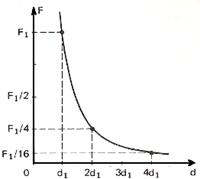
\includegraphics[width=0.5\linewidth]{Figuras/Ch05/coulomb3.jpg}}
}

\frame{
	\frametitle{Lei de Coulomb}
	\begin{block}{Operação vetorial}
		A força eletrostática é uma grandeza vetorial, portanto, possui módulo, direção e sentido.
		\begin{itemize}
			\item Devemos tomar cuidado quando fizermos operações básicas como soma e subtração de forças.
			\item Para determinarmos o módulo, a direção e o sentido de um vetor resultante, utilizamos a regra do paralelogramo.
		\end{itemize}
	\end{block}
}

\frame{
	\frametitle{Lei de Coulomb}
	\begin{block}{Operação vetorial - soma de vetores}
		\begin{itemize}
			\item Sejam $\vec{V_1}$ e $\vec{V_2}$  dois vetores. A soma desses vetores é um terceiro vetor, o vetor resultante $\vec{V}$:
			      $$\vec{V} = \vec{V_1} + \vec{V_2}$$
		\end{itemize}
	\end{block}
	
	\medskip

	\centering
	\begin{tikzpicture}
		\draw[-Latex] (0,0) -- node[midway,below] {$ \vec{V_2} $} ++(1,0);
		\draw[-Latex] (0,0) -- node[midway,left] {$ \vec{V_1} $} ++(0.4,1);
		
		\draw[-Latex] (0,0) -- node[midway,above] {$ \vec{V} $} ++(1.4,1);
		
		\draw[dashed] (0.4,1) -- ++(1,0);
		\draw[dashed] (1,0) -- ++(0.4,1);
		
		\coordinate (O) at (0,0);
		\coordinate (A) at (0.4,1);
		\coordinate (B) at (1,0);
		
		\path[gray]
		pic["$\alpha$" shift={(15pt,2pt)},draw,->,angle radius=0.8cm] {angle = B--O--A};
	\end{tikzpicture}
%	\centerline{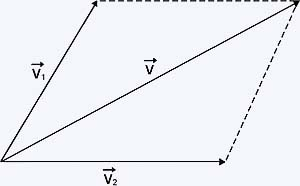
\includegraphics[width=0.4\linewidth]{Figuras/Ch05/soma.jpg}}
	\begin{block}{}
		$$\vec{V^2} = \vec{V_1^2} + \vec{V_2^2} + 2 \ \vec{V_1} \ \vec{V_2} \ \text{cos} \ \alpha$$
		onde $\alpha$ é o ângulo entre os dois vetores.
	\end{block}
}

\frame{
	\frametitle{Lei de Coulomb}
	\begin{block}{Operação vetorial - subtração de vetores}
		\begin{itemize}
			\item Consideremos os vetores $\vec{V_1}$ e $\vec{V_2}$. A subtração de vetores
			      $$\vec{V} = \vec{V_1} - \vec{V_2}$$
			      resulta em um terceiro vetor (chamado diferença), cujas propriedades são inferidas a partir da soma dos vetores $\vec{V_1}$ e ($-\vec{V_2}$).
		\end{itemize}
	\end{block}
	
	\medskip
	
	\centering
	\begin{tikzpicture}
	\draw[-Latex] (0,0) -- node[midway,below] {$ -\vec{V_2} $} ++(-1,0);
	\draw[-Latex] (0,0) -- node[midway,right] {$ \vec{V_1} $} ++(0.4,1);
	
	\draw[-Latex] (0,0) -- node[midway,below,xshift=-5pt] {$ \vec{V} $} ++(-0.6,1);
	
	\draw[dashed] (0.4,1) -- ++(-1,0);
	\draw[dashed] (-1,0) -- ++(0.4,1);
	\end{tikzpicture}

%	\centerline{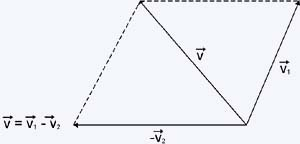
\includegraphics[width=0.4\linewidth]{Figuras/Ch05/subtracao.jpg}}
	\begin{block}{}
		O vetor $-\vec{V_2}$ tem módulo e direção iguais ao do vetor $\vec{V_2}$ mas tem o sentido oposto.
	\end{block}
}

\frame{
	\frametitle{Lei de Coulomb}
	\begin{block}{Exemplo \#01}
		Duas cargas puntiformes de valores \SI{3e-5}{\coulomb} e \SI{5e-6}{\coulomb} sofrem uma força de repulsão no vácuo. Sabendo que a constante eletrostática no vácuo é \SI{9e9}{\cons}, calcule a intensidade da força de repulsão entre as cargas, separadas por uma distância de \SI{0.15}{\meter}.
	\end{block}

	\vspace{1cm}

	\begin{block}{Resolução}
		\begin{align*}
			F 	&= K \ \dfrac{Q_1 \ Q_2}{d^2}\\
				&= \num{9e9} \ \dfrac{\num{3e-5} \cdot \num{5e-6}}{\num{0,15}^2} = \SI{60}{\newton}
		\end{align*}
	\end{block}
}

\frame{
	\frametitle{Lei de Coulomb}
	\begin{block}{Exemplo \#02}
		A figura abaixo mostra duas partículas positivamente carregadas situadas em pontos fixos no eixo $x$. As cargas são $q_1 = \SI{1.6e-19}{\coulomb}$ e $q_2 = \SI{3.2e-19}{\coulomb}$, e a distância entre as cargas é $ R = \SI{0.02}{\meter} $. Determine o módulo e a orientação da força eletrostática exercida pela partícula 2 sobre a 1.
	\end{block}

	\vspace{0.5cm}

%	\centering
%	\begin{tikzpicture}[scale=1]
%		\draw (-0.25,0) -- (1.25,0) node[right] {$ x $};
%		\filldraw[fill=gray] (0,0) circle (0.1) node {$ + $} (1,0) circle (0.1) node {$ - $};
%		\draw (0,0) +(120:0.2) node {$ q_1 $} (1,0) +(60:0.2) node {$ q_2 $};
%		\draw[|Latex-Latex] (0,-0.2) -- (1,-0.2);
%		\draw[-|] (0,-0.2) -- node[midway,fill=white] {$ R $} (1,-0.2);
%	\end{tikzpicture}

\centerline{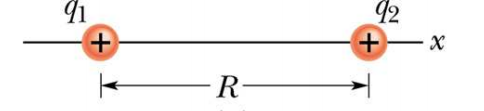
\includegraphics[width=0.4\linewidth]{Figuras/Ch05/exemplo02.PNG}}
}

\frame{
	\frametitle{Lei de Coulomb}
	\begin{block}{Resolução}
		\vspace{-0.2cm}
		\begin{align*}
		F_{12} 	&= K \ \dfrac{q_1 \ q_2}{r^2}\\
		&=\num{9e9} \ \dfrac{\num{1.6e-19} \cdot\num{3.2e-19}}{\num{0,02}^2} =\SI{1.15e-24}{\newton}
		\end{align*}
		
		A orientação que segue em relação ao sentido positivo de $x$ é de $\ang{180}$
	\end{block}
}

\frame{
	\frametitle{Lei de Coulomb}
	\begin{block}{Exemplo \#03}
		Determine a força resultante sobre a carga $q_1$ se for inserida uma carga $q_3$ no eixo $x$ entre as partículas 1 e 2. A partícula 3 tem carga $q_3 = \SI{-3.2e-19}{\coulomb} $ e está a uma distância $3/4R$ da partícula 1. Determine também a orientação da força resultante.
	\end{block}

	\vspace{0.5cm}
	
	\centering
	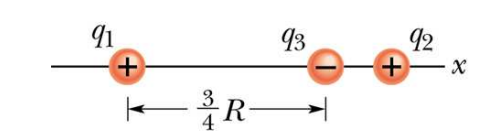
\includegraphics[width=0.4\linewidth]{Figuras/Ch05/exemplo03.PNG}
}

\frame{
	\frametitle{Lei de Coulomb}
	\begin{block}{Resolução}
		\vspace{-0.2cm}
		\begin{align*}
		F_{13}	&=K\dfrac{q_1\cdot q_3}{d^{2}}\\
		&=\num{9e9}\dfrac{\num{1.6e-19}\cdot\num{-3.2e-19}}{\num{0.015}^{2}}=\SI{-2.048e-24}{\newton}
		\end{align*}
		
		A força resultante é dada por $F_R = F_{12} + F_{13} = \SI{-8.98e-25}{\newton}$. A força resultante forma $\ang{0}$ com $x$.
	\end{block}
}

\section*{Exercícios}

\frame{
	\frametitle{Exercícios}
	\begin{block}{}
		01. Qual deve ser a distância entre a carga pontual $q_1 = \SI{26}{\micro\coulomb}$ e a carga pontual $q_2 =\SI{-47}{\micro\coulomb}$ para que a força resultante eletrostática entre as duas cargas tenha módulo de \SI{5.7}{\newton}?

		\vspace{0.3cm}

		02. (PUC-RJ) Duas esferas carregadas, afastadas de \SI{1}{\meter}, se atraem com uma força de \SI{720}{\newton}. Se uma esfera tem o dobro da carga da segunda, qual é a carga das duas esferas?

		\vspace{0.3cm}

%		03. (FUVEST-SP) A uma distância $d$ uma da outra, encontram-se duas esferinhas metálicas idênticas, de dimensões desprezíveis, com cargas $-Q$ e $+9Q$. Elas são postas em contato e, em seguida, colocadas à distância $2d$. Determine a razão entre os módulos das forças que atuam após o contato e antes do contato.
	\end{block}
}


\section*{Referências}

\frame{
	\frametitle{Referências e Exercícios Complementares}
	\begin{itemize}
		\item Física, Ciência e Tecnologia – Vol 3. PENTEADO, Paulo César M; TORRES, Carlos Magno A. Ed. Moderna (2006)
	\end{itemize}
	%\centering{\alert{Página 36 - \textbf{1.6.1 até 1.6.5, 1.6.17 até 1.6.19}}} \\
	%https://www.youtube.com/watch?v=IUgS7Uw-qBI
	\centering{\alert{Lista de exercícios 05}}
}